\documentclass[14pt, aspectratio=169, handout]{beamer}
\usetheme{Copenhagen}
\usecolortheme{seahorse}
\setbeamertemplate{navigation symbols}{}
\setbeamertemplate{headline}{}

%\usepackage{pgfpages}
%\pgfpagesuselayout{4 on 1}[a4paper, border shrink=5mm]

\usepackage{graphicx} % Required for inserting images
\usepackage{multicol}
%\usepackage{enumitem}
\usepackage{amsfonts}
\usepackage{amsmath}
\usepackage{xcolor}
\definecolor{myblue}{RGB}{0, 0, 255} 
\definecolor{mygreen}{RGB}{0, 180, 80}
\definecolor{myred}{RGB}{153, 0, 0}
\definecolor{myorange}{RGB}{255, 153, 51}
\definecolor{mypurple}{RGB}{102, 0, 204}
\usepackage{tikz}

%--- commands for transform arrows----------------
\newcommand{\transform}[2]{%
    \begin{tikzpicture}
        % Open circle
        \draw[thick] (0,0) circle (0.1);
        % Line with number above and adjustable length
        \draw[thick] (0.1,0) -- (#2,0) node[midway, above] {#1};
        % Filled circle
        \filldraw[thick] (#2,0) circle (0.1);
    \end{tikzpicture}%
}
\newcommand{\invtransform}[2]{%
    \begin{tikzpicture}
        % filled circle
        \filldraw[thick] (0,0) circle (0.1);
        % Line with number above and adjustable length
        \draw[thick] (0.1,0) -- (#2 -0.1,0) node[midway, above] {#1};
        % open circle
        \draw[thick] (#2,0) circle (0.1);
    \end{tikzpicture}%
}
\newcommand{\verticaltransform}[4]{%
    \begin{tikzpicture}
        % Open circle at the bottom with text below
        \filldraw[thick] (0,0) circle (0.1) node[below=3pt] {$#4$};
        % Vertical line with number on the left
        \draw[thick] (0,0.1) -- (0,#2 -0.1) node[midway, left] {#1};
        % Filled circle at the top with text above
        \draw[thick] (0,#2) circle (0.1) node[above=3pt] {$#3$};
    \end{tikzpicture}%
}
\newcommand{\verticalinvtransform}[4]{%
    \begin{tikzpicture}
        % Open circle at the bottom with text below
        \draw[thick] (0,0) circle (0.1) node[below=3pt] {$#4$};
        % Vertical line with number on the left
        \draw[thick] (0,0.1) -- (0,#2) node[midway, left] {#1};
        % Filled circle at the top with text above
        \filldraw[thick] (0,#2) circle (0.1) node[above=3pt] {$#3$};
    \end{tikzpicture}%
}

\definecolor{darkblue}{RGB}{0, 0, 139}
\definecolor{lightblue}{RGB}{173, 216, 230}

\title{SST1 Übungsstunde 11}
\author{Matteo Dietz}
\date{December 2024}

\begin{document}

\maketitle

\begin{frame}{Themenüberblick}
    \begin{itemize}
        \item \textbf{Diskrete Fouriertransformation (DFT)}
        \item[] Herleitung, Visualisierung, Matrixdarstellung
        \item[] 
        \item \textbf{Lineare und Zyklische Faltung}
        \item[] Zirkulante Matrizen
        \item[] Anwendungen der DFT auf LTI-Systeme
    \end{itemize}
\end{frame}

\begin{frame}{Aufgaben für diese Woche}
    \begin{itemize}
        \item[] \textbf{123}, \textbf{124}, \textbf{125}, \textbf{126}, \textbf{127}, \textbf{128}, \textbf{130}, \textbf{131}
        \item[] 
        \item[] Die \textbf{fettgedruckten} Übungen empfehle ich, weil sie wesentlich zu eurem Verständnis der Theorie beitragen und/oder sehr prüfungsrelevant sind.
        \item[] 
        \item[] Die DFT ist \textcolor{myred}{sehr wichtig}! Es kommt immer eine ganze Aufgabe dazu an der Prüfung. (25 / 100 Punkte)
    \end{itemize}
\end{frame}

\begin{frame}{DFT: Herleitung}
    \begin{itemize}
        \item Wir betrachten ein Signal $x[n]$ endlicher Länge $N$.
        \item Die DTFT des Signals ist
        $$\hat{x}(\theta) = \sum_{n=-\infty}^\infty x[n]e^{-2 \pi i \theta n} = \sum_{n=0}^{N-1} x[n]e^{-2 \pi i \theta n}$$
        \item $\hat{x}(\theta)$ ist kontinuierlich. Wir tasten $\hat{x}(\theta)$ im Frequenzbereich ab.
        $$\hat{x}[k] := \hat{x}\left(\frac{k}{N}\right) = \sum_{n=0}^{N-1} x[n]e^{-2 \pi i \frac{k}{N}} $$
    \end{itemize}
\end{frame}

\begin{frame}{Diskrete Fouriertransformation (DFT)}
    \fcolorbox{darkblue}{lightblue}{%
    \parbox{\dimexpr\linewidth-2\fboxsep-2\fboxrule\relax}{
    \vspace*{0.15cm}
    \begin{itemize}
        \item[] $(\textbf{DFT}) \hspace{40pt} \hat{x}[k] = \displaystyle\sum_{n=0}^{N-1} x[n]\omega_N^{kn} \hspace{50pt} \hat{x}[k+N] = \hat{x}[k]$
        \item[] $(\textbf{IDFT}) \hspace{36pt} x[n]=\displaystyle\frac{1}{N}\displaystyle\sum_{k=0}^{N-1} \hat{x}[k] \omega_N^{-kn} \hspace{42pt} x[n+N] = x[n]$
        \item[] wobei $\hspace{48pt} \omega_N = e^{-\frac{2 \pi i}{N}}$
    \end{itemize}
}}%
\end{frame}

\begin{frame}{DFT: Bemerkungen}
    \begin{enumerate}
    \item $\omega_N^l$ ist $N-$periodisch, denn: $\omega_N^{l + N} = e^{-\frac{2 \pi i}{N}(l+N)} = e^{-\frac{2 \pi i l}{N}} e^{- 2 \pi i} = \omega_N^l$
    \item[] 
    \item Es folgt: $\hat{x}[k+N] = \hat{x}[k]$. \textbf{Die DFT-Signale sind als $N-$periodisch zu interpretieren!}
    \item[] 
    \item \textbf{Abtastung im Frequenzbereich entspricht Periodisierung im Zeitbereich}.
\end{enumerate}
\end{frame}

\begin{frame}{DFT: Visualisierung}
    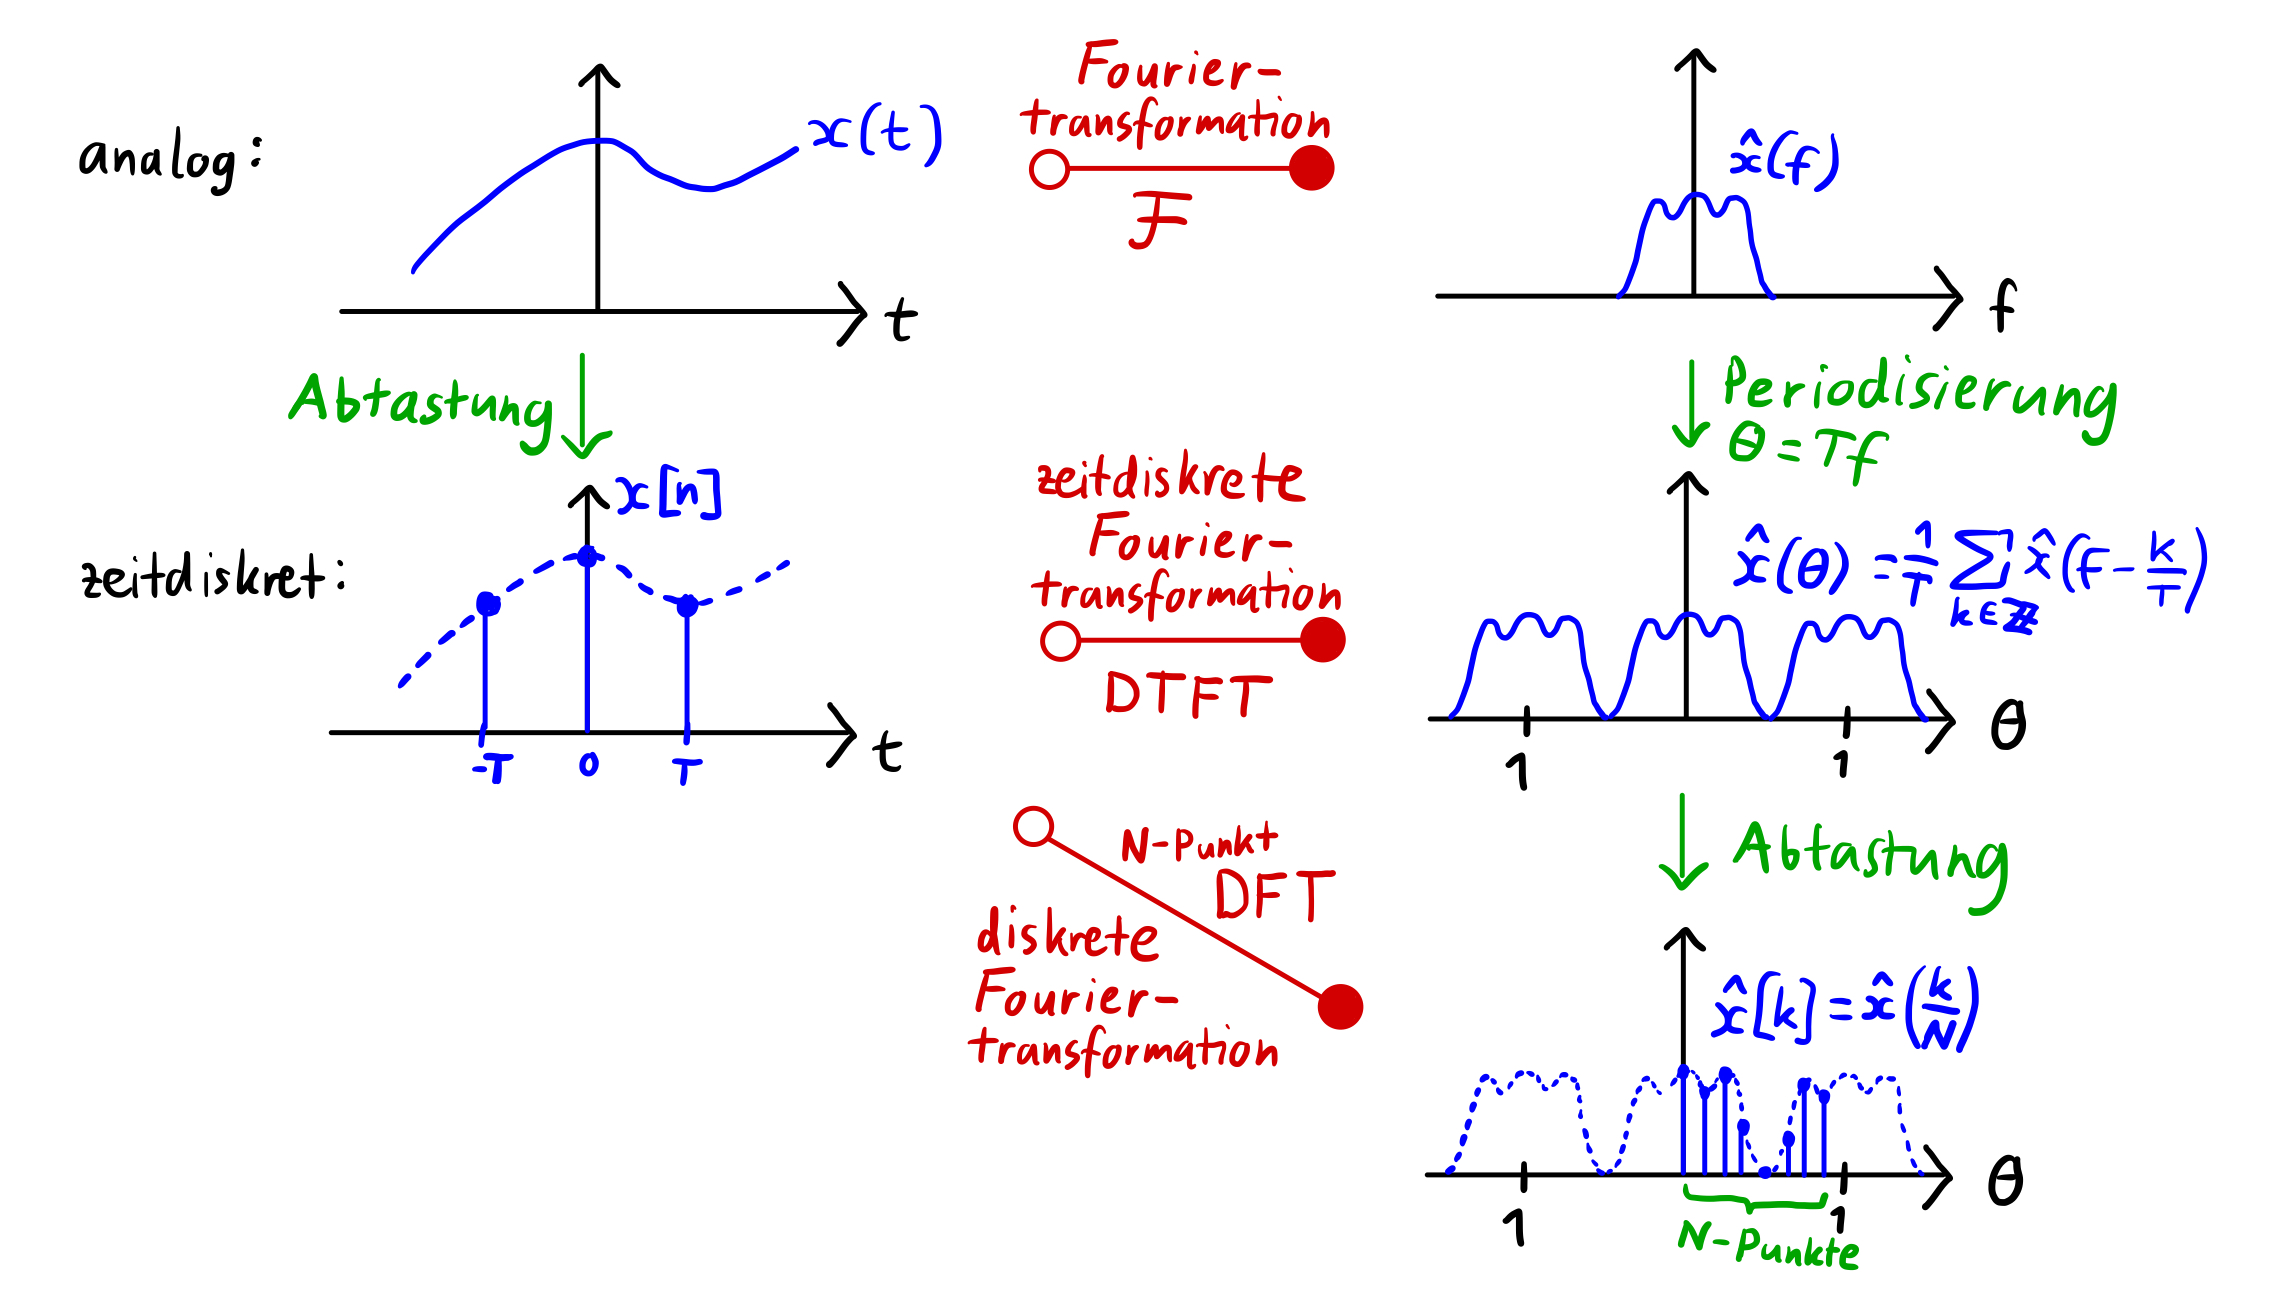
\includegraphics[width=0.95\linewidth]{figures/DFT_visuals.jpeg}
\end{frame}

\begin{frame}{DFT: Matrixdarstellung}
    Wir haben $\hat{x}[k] = \displaystyle\sum_{n=0}^{N-1} x[n]\omega_N^{kn}, \hspace{20pt} k \in \{ 0, \; 1, \; \dots, \; N-1 \}$ Somit:

$$\underbrace{\begin{bmatrix}
    \hat{x}[0] \\
    \hat{x}[1] \\
    \hat{x}[2] \\
    \vdots \\
    \hat{x}[N-1]
\end{bmatrix}}_{=: \hat{\mathbf{x}}} = \underbrace{\begin{bmatrix}
    1 & 1 & 1 & \cdots & 1 \\
    1 & \omega_N & \omega_N^2 & \cdots & \omega_N^{N-1} \\
    1 & \omega_N^2 & \omega_N^4 & \cdots & \omega_N^{2(N-1)} \\
    \vdots & \vdots & \vdots & \ddots & \vdots \\
    1 & \omega_N^{N-1} & \omega_N^{2(N-1)} & \cdots & \omega_N^{(N-1)^2}
\end{bmatrix}}_{\text{DFT-Matrix } F_N} \underbrace{\begin{bmatrix}
    x[0] \\
    x[1] \\
    x[2] \\
    \vdots \\
    x[N-1]
\end{bmatrix}}_{\mathbf{x}}$$

\end{frame}

\begin{frame}{DFT: Matrixdarstellung}
    
\fcolorbox{darkblue}{lightblue}{%
    \parbox{\dimexpr\linewidth-2\fboxsep-2\fboxrule\relax}{
        Somit erhalten wir: \\
        \noindent
        \begin{minipage}[t]{0.45\textwidth}
            \vspace*{0.1cm}
            \begin{itemize}
                \item[] \textbf{DFT}
                \item[] $\hat{\mathbf{x}} = F_N \mathbf{x}$
            \end{itemize}
            \vspace*{0.1cm}
        \end{minipage}%
        \hfill%
        \begin{minipage}[t]{0.45\textwidth}
            \vspace*{0.1cm}
            \begin{itemize}
                \item[] \textbf{IDFT}
                \item[] $\mathbf{x} = \frac{1}{N}F_N^H \hat{\mathbf{x}}$
            \end{itemize}
            \vspace*{0.1cm}
        \end{minipage}
    }%
}

\begin{itemize}
    \item[] 
    \item[] 
    \item[] Die Spalten von $F_N$ sind orthogonal aufeinander: $\langle \mathbf{f}_r, \; \mathbf{f}_s \rangle = \delta_{r,s}$
    \item[] 
    \item[] Es gilt $F_N F_N^H = N I_N$
\end{itemize}
\end{frame}

\begin{frame}{DFT: Entwicklung in eine ONB}
    Die DFT ist entspricht einer Entwicklung des Vektors $\mathbf{x}$ in eine orthonormale Basis (ONB) in $\mathbb{C}^N$:

$$\mathbf{x} = \underbrace{\frac{1}{N} \mathbf{F}_N^H \mathbf{F}_N}_{\mathbf{I}_N} \mathbf{x} = \frac{1}{N} \begin{bmatrix}
    \mathbf{f}_0 & \mathbf{f}_1 & \cdots & \mathbf{f}_{N-1}
\end{bmatrix} \begin{bmatrix}
    \mathbf{f}_0^H \\
    \mathbf{f}_1^H \\
    \vdots \\
    \mathbf{f}_{N-1}^H
\end{bmatrix} \mathbf{x} = \frac{1}{N} \sum_{l=0}^{N-1} \langle \mathbf{x}, \; \mathbf{f}_l \rangle \mathbf{f}_l$$
\end{frame}

\begin{frame}{DFT: Beispiel}
    Was ist die 2-Punkte DFT von $\mathbf{x} = \begin{bmatrix}
    x[0] \\
    x[1]
\end{bmatrix} = \begin{bmatrix}
    1 \\
    1
\end{bmatrix}$

$$F_2 = \begin{bmatrix}
    1 & 1 \\
    1 & \omega_2
\end{bmatrix} = \begin{bmatrix}
    1 & 1 \\
    1 & -1
\end{bmatrix}, \hspace{12pt} \text{weil } \omega_2 = e^{-\frac{2 \pi i}{2}} = -1, \hspace{12pt} \text{dann:}$$

$$ \hat{\mathbf{x}} = \begin{bmatrix}
    \hat{x}[0] \\
    \hat{x}[1]
\end{bmatrix} = \begin{bmatrix}
    1 & 1 \\
    1 & -1
\end{bmatrix} \begin{bmatrix}
    1 \\
    1
\end{bmatrix} = \begin{bmatrix}
    2 \\
    0
\end{bmatrix} $$
\end{frame}

\begin{frame}{Aufgabe 123}
    
\end{frame}

\begin{frame}{Zyklische Faltung}
    \fcolorbox{darkblue}{lightblue}{%
    \parbox{\dimexpr\linewidth-2\fboxsep-2\fboxrule\relax}{
    \vspace*{0.15cm}
    $$\vspace*{-0.5cm} x_3[l] = \sum_{n=0}^{N-1} x_1[n]x_2[l-n] = \sum_{n=0}^{N-1} x_1[l-n] x_2[n]$$
    $$\vspace*{-0.5cm}\verticaltransform{\text{DFT}}{1}{}{} \hspace{58pt}$$
    $$\hat{x}_3[k] = \hat{x}_1[k] \cdot \hat{x}_2[k]$$
}}%
\end{frame}

\begin{frame}{Zyklische Faltung: Bemerkungen}
    \begin{enumerate}
    \item \textbf{Elementweise Multiplikation im Frequenzbereich entspricht einer zyklischen Faltung im Zeitbereich}
    \item[] 
    \item $x_1[n], \; x_2[n], \; x_3[n]$ werden \textbf{$N-$periodisch fortgesetzt}, d.h. $x_2[l-n] = x_2[l-n+N] \neq 0$ ist möglich
    \item[]
    \item Zyklische Faltungen können schnell mittels FFT berechnet werden.
\end{enumerate}
\end{frame}

\begin{frame}{Lineare Faltung}
    $x_1[n]$ hat Länge $L$ und $x_2[n]$ hat Länge $P$. Wir wollen berechnen:
    $$ x_3[n] = \sum_{l=-\infty}^\infty x_1[l]\cdot x_2[n-l] = \sum_{l=-0}^{L-1} x_1[l]\cdot x_2[n-l] $$
    \begin{itemize}
        \item[] 
        \item[] 
        \item[] 
        \item[] 
        \item[] 
    \end{itemize}
\end{frame}

\begin{frame}{Lineare vs Zyklische Faltung: Aliasing}
    \noindent
    \begin{minipage}{0.6\textwidth}
        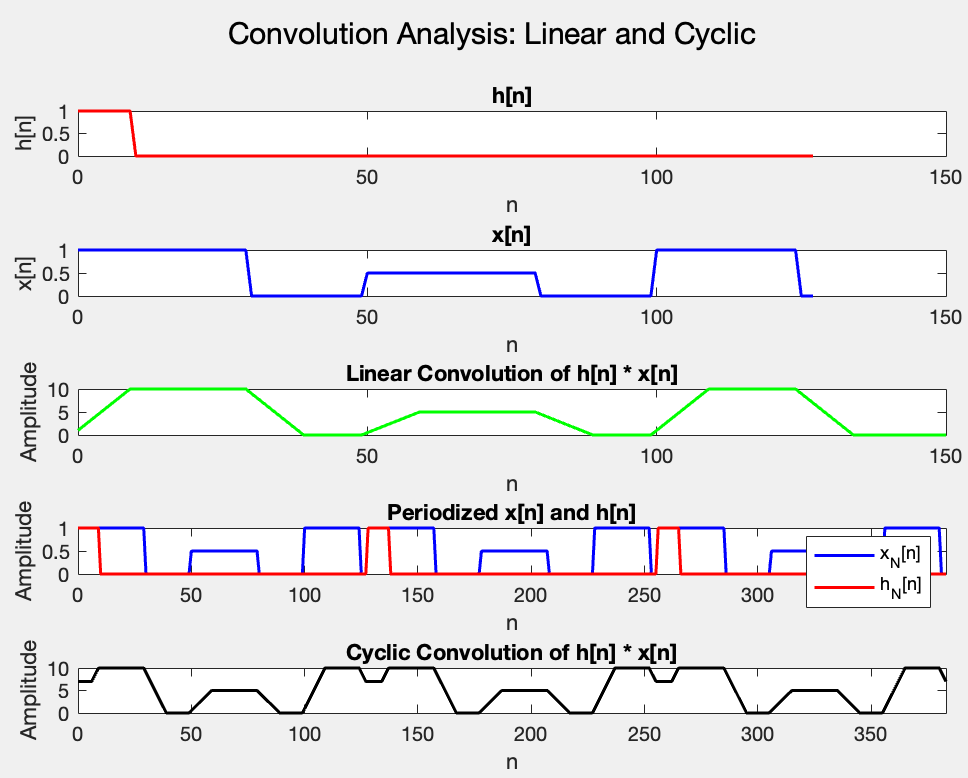
\includegraphics[width=\linewidth]{figures/conv_alias.png}
    \end{minipage}
    \hfill
    \begin{minipage}{0.35\textwidth}
        
    \end{minipage}
\end{frame}

\begin{frame}{Lineare vs Zyklische Faltung: kein Aliasing}
    \noindent
    \begin{minipage}{0.6\textwidth}
        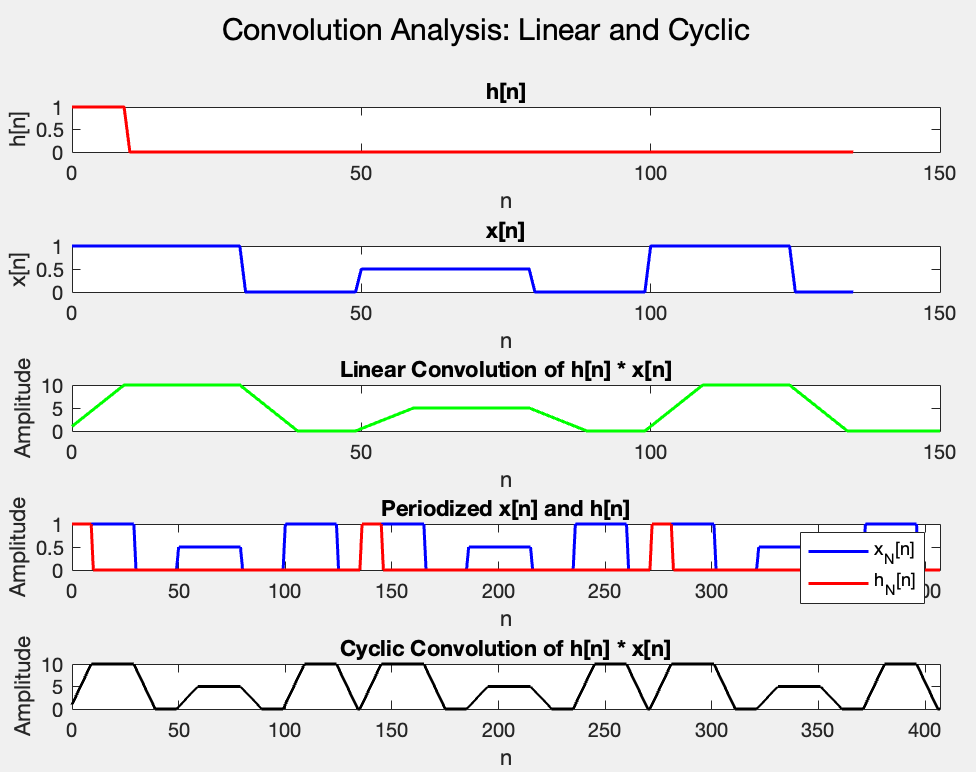
\includegraphics[width=\linewidth]{figures/conv_no_alias.png}
    \end{minipage}
    \hfill
    \begin{minipage}{0.35\textwidth}
        
    \end{minipage}
\end{frame}

\begin{frame}{Lineare Faltung: Kochrezept}
    \begin{enumerate}
    \item Zero-Padding (mit Nullen auffüllen) der Signale $x_1[n]$ und $x_2[n]$ auf die Länge $N \geq P + L - 1$
    \item[] 
    \item Berechnen der \textcolor{myred}{N-Punkte} DFT $\hat{x}_1[k]$ und $\hat{x}_2[k]$
    \item[] 
    \item Berechnen des punktweisen Produktes $\hat{x}_3[k] = \hat{x}_1[k] \cdot  \hat{x}_2[k]$
    \item[] 
    \item Inverse N-Punkte DFT von $\hat{x}_3[k]$
    \item[] Wir erhalten $\tilde{x}_3[n]$, die periodische Fortsetzung von $x_3[n]$
\end{enumerate}
\end{frame}

\begin{frame}{Zyklische Faltung: Matrixdarstellung}
\vspace*{-0.5cm}
\small{
    $$x_3[l] = \sum_{n=0}^{N-1} x_1[n]x_2[l-n] = \sum_{n=0}^{N-1} x_1[l-n] x_2[n]$$

\begin{align*}
    \underbrace{\begin{bmatrix}
        x_3[0] \\
        x_3[1] \\
        \vdots \\
        x_3[N-1]
    \end{bmatrix}}_{\mathbf{x}_3} &= \begin{bmatrix}
        x_2[0] & x_2[-1] & \cdots & x_2[-N+1] \\
        x_2[1] & x_2[0] & \cdots & x_2[-N+2] \\
        \vdots & \vdots & \ddots & \vdots \\
        x_2[N-1] & x_2[N-2] & \cdots & x_2[0]
    \end{bmatrix} \begin{bmatrix}
        x_1[0] \\
        x_1[1] \\
        \vdots \\
        x_1[N-1]
    \end{bmatrix} \\
    &\overset{\star}{=} \underbrace{\begin{bmatrix}
        x_2[0] & x_2[N-1] & \cdots & x_2[1] \\
        x_2[1] & x_2[0] & \cdots & x_2[2] \\
        \vdots & \vdots & \ddots & \vdots \\
        x_2[N-1] & x_2[N-2] & \cdots & x_2[0]
    \end{bmatrix}}_{\mathbf{X}_2} \underbrace{\begin{bmatrix}
        x_1[0] \\
        x_1[1] \\
        \vdots \\
        x_1[N-1]
    \end{bmatrix}}_{\mathbf{x}_1}
\end{align*}}
\end{frame}

\begin{frame}{Zyklische Faltung: Matrixdarstellung}
    \small{
    \begin{align*}
    \frac{1}{N}\mathbf{F}_N \mathbf{X}_2 \mathbf{F}_N^H &= \frac{1}{N} \begin{bmatrix}
        \hat{x}_2[0] & \hat{x}_2[0] & \cdots & \hat{x}_2[0] \\
        \hat{x}_2[1] & \hat{x}_2[1]\omega_N & \cdots & \hat{x}_2[1]\omega_N^{N-1} \\
        \hat{x}_2[2] & \hat{x}_2[2]\omega_N^2 & \cdots & \hat{x}_2[2]\omega_N^{2(N-1)} \\
        \vdots & \vdots & \ddots & \vdots \\
        \hat{x}_2[N-1] & \hat{x}_2[N-1]\omega_N^{N-1} & \cdots & \hat{x}_2[N-1]\omega_N^{(N-1)^2}
    \end{bmatrix} \mathbf{F}_N^H \\
    &= \frac{1}{N} \begin{bmatrix}
        \hat{x}_2[0] & & \mathbf{0} \\
        & \ddots & \\
        \mathbf{0} & & \hat{x}_2[N-1]
    \end{bmatrix} \underbrace{\begin{bmatrix}
        1 & 1 & 1 & \cdots & 1 \\
        1 & \omega_N & \omega_N^2 & \cdots & \omega_N^{N-1} \\
        1 & \omega_N^2 & \omega_N^4 & \cdots & \omega_N^{2(N-1)} \\
        \vdots & \vdots & \vdots & \ddots & \vdots \\
        1 & \omega_N^{N-1} & \omega_N^{2(N-1)} & \cdots & \omega_N^{(N-1)^2}
    \end{bmatrix}}_{\mathbf{F}_N} \mathbf{F}_N^H
\end{align*}}
\end{frame}

\begin{frame}{Zyklische Faltung: Matrixdarstellung}
    \begin{align*}
        &= \frac{1}{N} \begin{bmatrix}
        \hat{x}_2[0] & & \mathbf{0} \\
        & \ddots & \\
        \mathbf{0} & & \hat{x}_2[N-1]
    \end{bmatrix} N \mathbf{I}_N = \begin{bmatrix}
        \hat{x}_2[0] & & \mathbf{0} \\
        & \ddots & \\
        \mathbf{0} & & \hat{x}_2[N-1]
    \end{bmatrix} \\
    \text{Somit } \mathbf{X}_2 &= \frac{1}{N} \mathbf{F}_N^H  \begin{bmatrix}
        \hat{x}_2[0] & & \mathbf{0} \\
        & \ddots & \\
        \mathbf{0} & & \hat{x}_2[N-1]
    \end{bmatrix}   \mathbf{F}_N
    \end{align*}
\end{frame}

\begin{frame}{Bemerkungen}
    \begin{enumerate}
    \item Eigenvektoren einer zirkulanten Matrix $=$ Spalten der normalisierten DFT-Matrix $\frac{1}{\sqrt{N}}\mathbf{F}_N^H$
    \item[] Dazugehörige Eigenwerte sind durch die DFT der ersten Spalte der zirkulanten Matrix gegeben
    \item[] 
    \item Vgl. zeitkontinuierlicher Fall: $e^{2 \pi i f_0 t}$ Eigenfunktionen von LTI-Systemen sind und $\hat{h}(f)$ die dazugehörigen Eigenwerte
    \item[] 
    \item \textbf{Die zyklische Faltung wird durch die DFT diagonalisiert}.
\end{enumerate}
\end{frame}

\begin{frame}{Anwendung DFT auf LTI-Systeme}
    $$\vspace*{-0.45cm}\mathbf{y} = \mathbf{H}\mathbf{x} =  \frac{1}{N} \mathbf{F}_N^H  \begin{bmatrix}
    \hat{h}[0] & & \mathbf{0} \\
    & \ddots & \\
    \mathbf{0} & & \hat{h}[N-1]
\end{bmatrix} \mathbf{F}_N \mathbf{x}$$
$$\vspace*{-0.45cm}\verticaltransform{\text{DFT}}{1}{}{} \hspace{7.5cm}$$
$$\mathbf{F}_N \mathbf{y} = \underbrace{\frac{1}{N} \mathbf{F}_N \mathbf{F}_N^H}_{\mathbf{I}_N}  \begin{bmatrix}
    \hat{h}[0] & & \mathbf{0} \\
    & \ddots & \\
    \mathbf{0} & & \hat{h}[N-1]
\end{bmatrix} \hat{\mathbf{x}} = \begin{bmatrix}
    \hat{h}[0] \hat{x}[0] \\
    \hat{h}[1] \hat{x}[1] \\
    \vdots \\
    \hat{h}[N-1] \hat{x}[N-1]
\end{bmatrix}$$
\end{frame}

\begin{frame}{LTI-Systeme kommutieren}
\small{
    \begin{align*}
    \mathbf{H}_1 \mathbf{H}_2 &= \frac{1}{N} \mathbf{F}_N^H \begin{bmatrix}
        \hat{h}_1[0] & & \mathbf{0} \\
        & \ddots & \\
        \mathbf{0} & & \hat{h}_1[N-1]
    \end{bmatrix} \underbrace{\mathbf{F}_N \frac{1}{N} \mathbf{F}_N^H}_{\mathbf{I}_N}  \begin{bmatrix}
        \hat{h}_2[0] & & \mathbf{0} \\
        & \ddots & \\
        \mathbf{0} & & \hat{h}_2[N-1]
    \end{bmatrix}\mathbf{F}_N \\
    &= \frac{1}{N} \mathbf{F}_N^H \begin{bmatrix}
        \hat{h}_1[0]\hat{h}_2[0] & & \mathbf{0} \\
        & \ddots & \\
        \mathbf{0} & & \hat{h}_1[N-1]\hat{h}_2[N-1]
    \end{bmatrix}\mathbf{F}_N \\
    &= \frac{1}{N} \mathbf{F}_N^H \begin{bmatrix}
        \hat{h}_2[0] & & \mathbf{0} \\
        & \ddots & \\
        \mathbf{0} & & \hat{h}_2[N-1]
    \end{bmatrix} \underbrace{\mathbf{F}_N \frac{1}{N} \mathbf{F}_N^H}_{\mathbf{I}_N}  \begin{bmatrix}
        \hat{h}_1[0] & & \mathbf{0} \\
        & \ddots & \\
        \mathbf{0} & & \hat{h}_1[N-1]
    \end{bmatrix} \mathbf{F}_N \\
    &= \mathbf{H}_2 \mathbf{H}_1
\end{align*}}
\end{frame}

\begin{frame}{Prüfungsaufgabe: Sommer 2020, Aufgabe 3.a) und b)}
    
\end{frame}

\end{document}